% Chapter Template

\chapter{Local-timed Negotiations}

\section{Introduction}

Computing systems often consist of multiple components that interact with each other to execute a task. For instance, ATMs, online banking platforms, and e-commerce retailers all maintain a coordinated conversation between customers at the front end and data servers at the back end. In many cases, these interactions need to meet timing constraints---for example, a one-time password (OTP) times out if it is not entered within a short window. Hence, when specifying such interactions, it becomes important to accurately describe the interplay between concurrency and timing.

In \cite{DBLP:journals/acta/DeselEH19,DBLP:conf/concur/EsparzaD13}, Esparza et al. introduced \textit{negotiations} as a model for describing computations involving a set of agents. Conventional automata-theoretic models focus on states and transitions, and specify how local states of agents determine global behaviours. In negotiations, the basic building blocks are the interactions between the agents. Individual interactions between a set of agents are called \emph{atomic negotiations}. After each atomic negotiation, the participating agents collectively agree on an outcome and move on to participate in other atomic negotiations. Apart from providing an attractive alternative perspective for modelling concurrent systems, negotiations also admit efficient analysis procedures. For some subclasses, interesting properties can be analyzed in polynomial-time~\cite{DBLP:journals/lmcs/EsparzaKMW18,DBLP:conf/lics/EsparzaMW17}.

The basic negotiation model does not have any mechanism to incorporate timing constraints between interactions. In~\cite{DBLP:conf/fossacs/AkshayGHM20} a notion of timed negotiations has been proposed, where every outcome is associated with an interval representing the minimum and maximum amount of time required for the interaction to conclude. The work focuses on computing the minimum and maximum execution times for the overall negotiation to complete. This model cannot express constraints on the time between different atomic negotiations. For this, we introduce clocks, as defined in timed automata~\cite{DBLP:journals/tcs/AlurD94}.

\noindent\emph{Related work.} A local-time semantics was proposed in
the context of networks of timed automata
in~\cite{DBLP:conf/concur/BengtssonJLY98}. Recently, the semantics has
been applied to the zone-based verification of
reachability~\cite{DBLP:conf/concur/GovindHSW19,DBLP:conf/lics/0001HSW22}
and B\"uchi reachability
properties~\cite{DBLP:conf/concur/HerbreteauSW22}. Local-time
semantics in timed automata has been investigated as a basis for
applying partial-order methods.  In our current work, we consider
local-time semantics as the starting point and make synchronization an
option that can be specified explicitly. This allows more independence
between the agents and keeps the concurrency between actions of
disjoint sets of agents.

Models mixing concurrency and timing have been widely studied: time
Petri nets~\cite{10.5555/907383}, timed-arc Petri
nets~\cite{DBLP:conf/apn/Hanisch93}, time-constrained message sequence
charts~\cite{DBLP:conf/concur/AkshayMK07} to name a few. Each model
offers a different view of the computation. To our knowledge, a notion
of a real-time has not yet been considered for negotiations.
With similar motivations as local-time semantics, a notion of a
partial-order semantics has been studied for networks of timed
automata~\cite{DBLP:journals/tcs/LugiezNZ05} as well as time Petri
nets~\cite{DBLP:conf/formats/ChatainJ05,DBLP:conf/apn/ChatainJ06}. This
semantics can be used to compute finite unfoldings which preserve the
concurrency and reachability information
concisely~\cite{DBLP:conf/atva/CassezCJ06,DBLP:conf/atva/BouyerHR06}.

\begin{figure}[t]
  \centering
  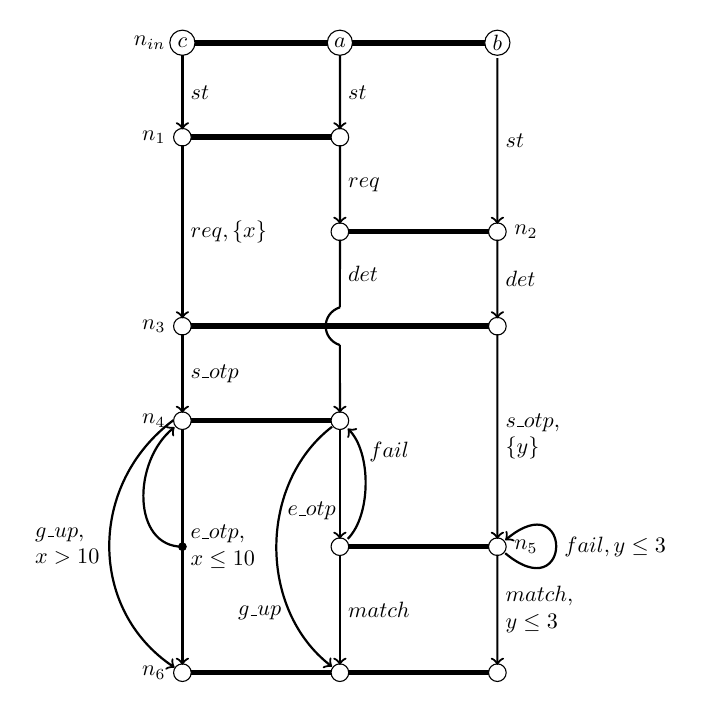
\begin{tikzpicture}[scale=0.8, every node/.style={transform shape}]

\begin{scope}[line width=2pt]
  \draw (0.,0) node [left] {$n_{in}\,\,$} -- (5,0); \draw (0.,-1.5)
  node [left] {$n_{1}\,\,$} -- (2.5,-1.5); \draw (2.5,-3) -- (5,-3)
  node [right] {$\,\,n_{2}$}; \draw (0.,-4.5) node [left]
  {$n_{3}\,\,$} -- (5,-4.5); \draw (0.,-6) node [left] {$n_{4}\,\,$}
  -- (2.5,-6); \draw (2.5,-8) -- (5,-8) node [right] {\,\,$n_{5}$};
  \draw (0.,-10) node [left] {$n_{6}\,\,$} -- (5,-10);
\end{scope}

\begin{scope}[fill=white]
  \filldraw (0,0) circle (2mm) node (nic) {$c$}; \filldraw (2.5,0)
  circle (2mm) node (nia) {$a$}; \filldraw (5,0) circle (2mm) node
  (nib) {$b$};

  \filldraw (0,-1.5) circle (1.4mm) node (n1c) {}; \filldraw
  (2.5,-1.5) circle (1.4mm) node (n1a) {};

  \filldraw (2.5,-3) circle (1.4mm) node (n2a) {}; \filldraw (5,-3)
  circle (1.4mm) node (n2b) {};

  \filldraw (0,-4.5) circle (1.4mm) node (n3c) {}; \filldraw (5,-4.5)
  circle (1.4mm) node (n3b) {};

  \filldraw (0,-6) circle (1.4mm) node (n4c) {}; \filldraw (2.5,-6)
  circle (1.4mm) node (n4a) {};

  \filldraw (2.5,-8) circle (1.4mm) node (n5a) {}; \filldraw (5,-8)
  circle (1.4mm) node (n5b) {};

  \filldraw (0,-10) circle (1.4mm) node (n6c) {}; \filldraw (2.5,-10)
  circle (1.4mm) node (n6a) {}; \filldraw (5,-10) circle (1.4mm) node
  (n6b) {};

  \filldraw [fill=black] (0,-8) circle (0.6mm) node (v1) {};

\end{scope}

\begin{scope}[thick,->]

  \draw (nic) -- (n1c) node [right, midway] {$st$}; \draw (n1c) --
  (n3c) node [right, midway] {$req, \{x\}$}; \draw (n3c) -- (n4c) node
  [right, midway] {$s\_otp$}; \draw (n4c) -- (n6c) node [right, text
  width = 1.2 cm, midway] {$e\_otp,$ $x\leq10$}; \draw (0,-8)
  .. controls (-0.8,-8) and (-0.8,-6.65) .. (n4c) node [left, midway]
  {};

  \draw (nia) -- (n1a) node [right, midway] {$st$}; \draw (n1a) --
  (n2a) node [right, midway] {$req$}; \draw (2.5,-4.8) -- (n4a); \draw
  (n4a) -- (n5a) node [left=-0.3cm, text width = 1 cm, near end]
  {$e\_otp$}; \draw (n5a) -- (n6a) node [right, text width = 1 cm,
  midway] {$match$}; \draw (n5a) .. controls (3,-7.5) and (3,-6.5)
  .. (n4a) node [right, near end] {$fail$}; \draw (n4a) .. controls
  (1.2,-7) and (1.2,-9) .. (n6a) node [left=-0.3cm, text width = 1 cm,
  near end] {$g\_up$};

  \draw (nib) -- (n2b) node [right, midway] {$st$}; \draw (n2b) --
  (n3b) node [right, midway] {$det$}; \draw (n3b) -- (n5b) node
  [right, text width = 1 cm, midway] {$s\_otp,$ $\{y\}$}; \draw (n5b)
  -- (n6b) node [right, text width = 1 cm, midway] {$match,$
    $y\leq3$}; \draw (n5b) .. controls (6.2,-9) and (6.2,-7) .. (n5b)
  node [right, midway] {$fail, y\leq3$};

  \draw (n4c) + (-0.14,0.01) .. controls (-1.5,-7) and (-1.5,-9)
  .. (n6c) node [left=-0.2cm, text width = 1.25 cm, midway] {$g\_up,$
    $x > 10$};

\end{scope}

\draw [thick] (n2a) -- (2.5,-4.2) node [right, midway] {$det$}; \draw
[thick] (2.5,-4.2) .. controls (2.2,-4.3) and (2.2,-4.7)
.. (2.5,-4.8);
\end{tikzpicture}
\caption{A local-timed negotiation modeling a transaction between a
  customer, an ATM and a bank}
\label{fig:ATM}
\end{figure}

\smallskip

\noindent\emph{A motivating example.} We use the example in Figure~\ref{fig:ATM} to introduce our model informally.  Consider a time-constrained transaction in an ATM machine ($a$), where a customer ($c$) wants to reset her ATM PIN via an OTP received from her bank ($b$).  Here, $a$, $c$, and $b$ are the \emph{agents} in the system. Their direct interactions are represented by thick horizontal lines, called nodes. After each interaction, the participating agents decide on an outcome, represented by arrows. Initially, all agents are in the node $n_{in}$ node. They choose the outcome $st$ to start the transaction. Agents $a$ and $c$ go to node $n_1$ and $b$ goes to $n_2$.The customer gives her card details and requests for a PIN change in the ATM at  node $n_1$ by choosing the outcome $req$. At $n_2$, the ATM conveys this request to the bank and sends the details through the outcome $det$. The bank and the customer talk to each other at $n_3$, and $b$ sends an OTP to the customer through the outcome $s\_otp$. At $n_4$, the customer enters the OTP in the ATM. After entering the OTP, shown by the outcome $e\_otp$ the customer is ready to engage with the ATM either at $n_4$ or at $n_6$, represented by the non-deterministic arc leading to $n_4$ and $n_6$.
The ATM talks to the bank at $n_5$ to check the OTP. If it matches,
the ATM goes to $n_6$, otherwise it goes back to $n_4$.

In this example, we model two time constraints. The bank would like to ensure that at most $3$ time units elapse between the sending of the OTP and the final match. This is achieved by resetting a local clock $y$ of the bank and checking that $y \le 3$ at the outcome \emph{match}.  On the other hand, the customer wants at most $10$ time units to have elapsed between initiating the request and completing the transaction. This is achieved by resetting a local clock $x$ at the outcome $req$ and checking that $x \le 10$ at the outcome $e\_otp$. If more than $10$ units elapse, the customer gives up, fires the outcome $g\_up$.  It is natural to imagine that clocks $x$ and $y$ are local to the customer and to the bank and that they may evolve at different rates.  We formalize this behaviour in terms of our local-time semantics. However, as we will see later, in certain interactions, it is useful to force the agents to synchronize their local times. Combining the concurrency present in negotiations with timing constraints and a mechanism to synchronize local times makes the model surprisingly powerful.

\section{Definition}

For a finite set $S$ we write $\Pp(S)$ for the power set containing all subsets of $S$. Let $\Rpos$ denote the set of non-negative reals, and $\Nat$ the set of natural numbers. For a real number $\alpha \in \Rpos$, we write $\lfloor \alpha \rfloor$ for the greatest integer smaller than or equal to $\alpha$, and $\{ \alpha \}$ for the fractional part $\alpha - \lfloor \alpha \rfloor$. A \emph{clock} is a real-valued variable whose values increase along with time and get updated during transitions (exact semantics comes later). Let $X$ be a set of clocks. A \emph{guard} over $X$ is a conjunction of clock constraints of the form $x \bowtie c$ where $x \in X$, $\bowtie \in \{ <, \le, =, >, \ge \}$ and $c \in \Nat$. We write $\Phi(X)$ for the set of guards over $X$.

\begin{definition}[Local-timed negotations]\label{def:local-timed-negot}
Let $P$ be a finite set of agents, $\Sigma$ a finite set of outcomes and $X$ a finite set of clocks. We assume that $X$ is partitioned as $\{ X_p \}_{p \in P}$ with $X_p$ being the \emph{local clocks} for agent $p$. Further, we associate a special clock $t_p$ to each agent $p$, called its \emph{reference clock}. This clock is neither used in a guard nor reset. We denote $T$ to be the set $\{ t_p \mid p \in P \}$ of reference clocks. A \emph{local-timed negotiation} $\Nn$ is given by a tuple $(N, \dom, \delta, Sync)$ where
\begin{itemize}
	\item $N$ is a finite set of nodes (also called atomic negotiations); there is a special initial node $n_{in} \in N$,
	\item $\dom: N \to \Pp(P)$ maps each node to a non-empty subset of agents; we assume $\dom(n_{in}) = P$; for $p \in P$, we let $N_p := \{ n \in N \mid p \in \dom(n) \}$
	\item $\delta = \{\delta_p\}_{p \in P}$ is a tuple of transition relations, one for each agent, where $\delta_p: N_p \times \Sigma \to \Phi(X) \times \Pp(N_p) \times \Pp(X_p)$ maps each node-outcome pair $(n, a)$ to a guard $g \in \Phi(X)$, a set of nodes $M \incl N_p$ that $p$ becomes ready to engage in after this outcome, and a set $Y \incl X_p$ of clocks that get reset; we will call node-outcome pairs $(n, a)$ as \emph{locations} (as in \cite{DBLP:conf/lics/EsparzaMW17} for untimed negotiations), 
	\item $\Sync \incl N$ is a subset of \emph{synchronizing nodes}.
\end{itemize}
\end{definition}

Figure~\ref{fig:ATM} gives an example of a local-timed negotiation over agents $P = \{c, a, b\}$. The set of nodes is given by $N = \{n_{in}, n_1, \dots, n_6\}$.  The domain $\dom(n)$ of a node $n$ is represented by the ``circles'' in each node: for instance, $\dom(n_1) = \{c, a\}$ and $\dom(n_2) = \{a, b\}$. Agent $c$ has a local clock $x$, and agent $b$ has a local clock $y$. As an example of a transition for agent $c$, we have $\delta_c(n_4, e\_otp) = (x \le 10, \{n_4, n_6\}, \{\})$. There is a guard $x \le 10$, the agent is ready to engage in $n_4$ and $n_6$ after the outcome, and no clock is reset. In this example, $\Sync$ is empty. 

\smallskip
\noindent \emph{Semantics.} The semantics of a negotiation is described using \emph{markings} and \emph{valuations}.  A marking $C$ is a function assigning each agent $p$ to a subset of $N_p$. It gives the set of nodes that each agent is ready to engage in. A valuation $v: X \cup T \to \Rpos$ maps every clock (including reference clocks) to a non-negative real such that $v(x) \le v(t_p)$ for all $x \in X_p$, and all agents $p \in P$. The interpretation is that clocks in $X_p$ move at the same pace as $t_p$, the local reference clock. Since $t_p$ is never reset it gives the local time at agent $p$. For a constraint $x \bowtie c$ we say $v \models x \bowtie c$ if $v(x) \bowtie c$. We say $v$ satisfies guard $g \in \Phi(X)$, written as $v \models g$, if $v$ satisfies every atomic constraint appearing in $g$.

A \emph{local-delay} $\Delta \in \Rpos^{|P|}$ is a vector of non-negative reals, giving a time elapse for each agent. Each agent can have a different time elapse.  Given a valuation $v$ and a local-delay $\Delta$, we write $v + \Delta$ for the valuation obtained as follows: for each agent $p \in P$, we have $(v + \Delta)(y) = v(y) + \Delta(p)$ for every $y \in \{t_p\} \cup X_p$. Notice that all clocks within a process move at the same rate as its reference clock. However, the reference clocks of different agents can move at different speeds. For a set of clocks $Y \incl X$, we denote by $v[Y]$ the valuation satisfying $v[Y](y) = 0$ if $y \in Y$ and $v[Y](y) = v(y)$ otherwise. 

A configuration is a pair $(C, v)$ consisting of a marking $C$ and a valuation $v$. The \emph{initial configuration} $(C_0, v_0)$ contains a marking $C_0$ which maps every agent to $n_{in}$ and valuation $v_0$ maps all clocks to $0$. We write $(C, v) \xra{\Delta} (C, v+\Delta)$ for the local-delay transition $\Delta$ at configuration $(C, v)$. For the negotiation in Figure~\ref{fig:ATM}, an example of a configuration is $(\bar{C}, \bar{v})$ with $\bar{C}(c) = \{ n_1 \}$, $\bar{C}(a) = \{n_1\}$ and $\bar{C}(b) = \{n_2\}$ and $\bar{v}(t_c) = \bar{v}(x) = 2$, $\bar{v}(t_a) = 1$ and $\bar{v}(t_b) = \bar{v}(y) = 3$. Suppose $\Delta = (c \mapsto 1, a \mapsto 0, b \mapsto 2)$, then $\bar{v} + \Delta$ maps $t_c$ and $x$ to $3$, and $t_b$ and $y$ to $5$ whereas $t_a$ remains $1$. 

A location $t = (n, a)$ can be executed at a configuration $(C, v)$ leading to a configuration $(C', v')$, written as $(C, v) \xra{t} (C', v')$, provided there is an entry $\delta_p(n, a) = (g_p, M_p, Y_p)$ for all $p \in \dom(n)$ such that:
\begin{itemize}
	\item \emph{current marking enables the negotiation:} $n \in C(p)$ for all $p \in \dom(n)$,
	\item \emph{synchronization condition is met:} if $n \in Sync$, then $v(t_p) = v(t_q)$ for all $p, q \in \dom(n)$,
	\item \emph{guard is satisfied}: $v \models g_p$ for all $p \in \dom(n)$,
	\item \emph{target marking is correct}: $C'(p) = M_p$ for all $p \in \dom(n)$, $C'(p) = C(p)$ for $p \notin \dom(n)$,
	\item \emph{resets are performed}: $v'(y) = 0$ for $y \in \bigcup_{p \in \dom(n)} Y_p$
\end{itemize}

For an example, consider Figure~\ref{fig:ATM} again and a configuration $(C^1, v^1)$ with $C^1:= (\{n_4, n_6\}, \{n_4\}, \{n_6\})$ and $v^1: \langle t_c = 10, x = 5, t_a = 20, t_b = 5, y = 1 \rangle$. Location $(n_4, e\_otp)$ is enabled leading to a configuration $(C^2, v^2)$ where $C^2 := ( \{n_4, n_6\}, \{n_6\}, \{n_6\})$ and $v^2 = v^1$, as there are no resets in this location.  

We call $(C, v) \xra{\Delta} (C, v + \Delta) \xra{t} (C', v')$ a \emph{small step} and write this as $(C, v) \xra{\Delta, t} (C', v')$ for conciseness. A \emph{run} is a sequence of small steps starting from the initial configuration. We say that a location $t = (n,a)$ is \emph{reachable} (in the negotiation) if there is a run containing a small step that executes $t$. The \emph{untimed language} of the negotiation $\Nn$ is the set of all words $w:= a_0a_1\dots a_n \in \Sigma^*$ such that there is a run $(C_0, v_0)\xra{\Delta_0, a_0} (C_1, v_1) \xra{\Delta_1, a_1} \cdots\xra{\Delta_n, a_n} (C_{n+1}, v_{n+1})$. 

\emph{Location-reachability problem.} We are interested in the following question: given a local-timed negotiation $\Nn$ and a location $t =(n,a)$ as inputs, is $t$ reachable in $\Nn$?

\subsection{Examples}

In the example of Figure~\ref{fig:ATM}, we have seen how
local-clocks can be used to constrain interactions. We will now see
some examples that show some interesting mechanics of synchronized
interactions. The negotiation in the left of Figure~\ref{fig:k-vendor} has three agents $p, q,
v$. The outcome at node $n_1$ results in a non-deterministic choice
for agent $q$: the agent may either decide to talk with $p$ at $n_3$
or with $v$ at $n_2$. Suppose at $n_3$, agent $p$ wants to make sure
that $q$ has arrived at $n_3$ after talking to $v$. We can imagine
that $v$ is a vendor, and $p$ wants to ensure that $q$ has indeed
met the vendor between their meetings at $n_1$ and $n_3$. To do this,
we make use of timing and synchronization constraints as
follows.

\begin{figure}[t]
\centering
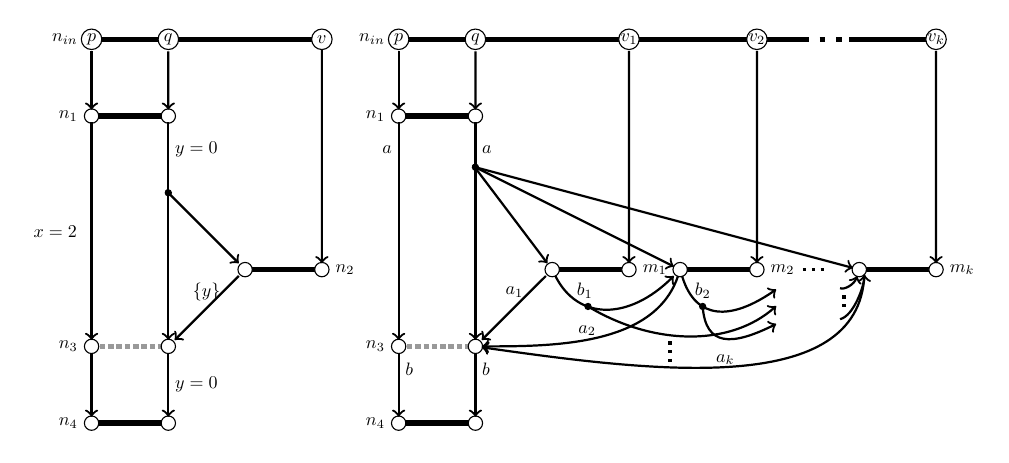
\begin{tikzpicture}[scale=0.65, every node/.style={transform shape}]

\begin{scope}[shift={(-6,0)}]
\begin{scope}[line width=2pt]
\draw (0.,0) node [left] {$n_{in}\,\,$} -- (4.5,0);
\draw (0,-1.5) node [black, left, opacity=1] {$n_1\,\,$} -- (1.5,-1.5);
\draw (3,-4.5)  -- (4.5,-4.5) node [right] {\,\,$n_2$};
\draw [densely dotted, opacity=0.4] (0,-6) node [black, left, opacity=1] {$n_3\,\,$} -- (1.5,-6);
\draw (0,-7.5) node [left] {$n_{4}\,\,$} -- (1.5,-7.5);
\end{scope}

\filldraw [fill=white]  (0,0)  circle (2mm) node 		(nip) {$p$};
\filldraw [fill=white]  (1.5,0)  circle (2mm) node 		(niq) {$q$};
\filldraw [fill=white]  (4.5,0)  circle (2mm) node 		(niv) {$v$};

\filldraw [fill=white]  (0,-1.5)  circle (1.4mm) node 	(n1p) {};
\filldraw [fill=white]  (1.5,-1.5)  circle (1.4mm) node (n1q) {};

\filldraw [fill=black]  (1.5,-3) circle (.6mm) node		(virt) {};

\filldraw [fill=white]  (3,-4.5)  circle (1.4mm) node 	(n21) {};
\filldraw [fill=white]  (4.5,-4.5)  circle (1.4mm) node (n2v) {};

\filldraw [fill=white]  (0,-6)  circle (1.4mm) node 	(n3p) {};
\filldraw [fill=white]  (1.5,-6)  circle (1.4mm) node 	(n3q) {};

\filldraw [fill=white]  (0,-7.5)  circle (1.4mm) node 	(nfp) {};
\filldraw [fill=white]  (1.5,-7.5)  circle (1.4mm) node (nfq) {};


\begin{scope}[thick,->]

\draw (nip) -- (n1p);
\draw (n1p) -- (n3p) node [midway, left, text width = 1cm] {$x=2$};
\draw (n3p) -- (nfp) node [midway, left] {};

\draw (niq) -- (n1q);
\draw (n1q) -- (n3q) node [very near start, right] {$y=0$};
\draw (virt) + (-.05,.05) -- (n21);
\draw (n21) -- (n3q) node [midway, above] {$\{y\}$};
\draw (n3q) -- (nfq) node [midway, right, text width = 1cm] {$y=0$};

\draw (niv) -- (n2v);

\end{scope}
\end{scope}

\begin{scope}[line width=2pt]
\draw (0.,0) node [left] {$n_{in}\,\,$} -- (7.9,0);
\draw (8.8,0) node [left] {} -- (10.5,0);
\draw (0,-1.5) node [black, left, opacity=1] {$n_1\,\,$} -- (1.5,-1.5);
\draw (3,-4.5)  -- (4.5,-4.5) node [right] {\,\,$m_1$};
\draw (5.5,-4.5)  -- (7,-4.5) node [right] {\,\,$m_2$};
\draw (9,-4.5)  -- (10.5,-4.5) node [right] {\,\,$m_k$};
\draw [densely dotted, opacity=0.4] (0,-6) node [black, left, opacity=1] {$n_3\,\,$} -- (1.5,-6);
\draw (0,-7.5) node [left] {$n_{4}\,\,$} -- (1.5,-7.5);
\end{scope}

\filldraw [fill=white]  (0,0)  circle (2mm) node 		(nip) {$p$};
\filldraw [fill=white]  (1.5,0)  circle (2mm) node 		(niq) {$q$};
\filldraw [fill=white]  (4.5,0)  circle (2mm) node 		(niv) {$v_1$};
\filldraw [fill=white]  (7,0)  circle (2mm) node 		(niv2) {$v_2$};
\filldraw [fill=white]  (10.5,0)  circle (2mm) node 		(nivk) {$v_k$};

\filldraw [fill=white]  (0,-1.5)  circle (1.4mm) node 	(n1p) {};
\filldraw [fill=white]  (1.5,-1.5)  circle (1.4mm) node (n1q) {};

\filldraw [fill=black]  (1.5,-2.5) circle (.6mm) node		(virt) {};

\filldraw [fill=white]  (3,-4.5)  circle (1.4mm) node 	(n21) {};
\filldraw [fill=white]  (4.5,-4.5)  circle (1.4mm) node (n2v) {};

\filldraw [fill=white]  (0,-6)  circle (1.4mm) node 	(n3p) {};
\filldraw [fill=white]  (1.5,-6)  circle (1.4mm) node 	(n3q) {};

\filldraw [fill=white]  (0,-7.5)  circle (1.4mm) node 	(nfp) {};
\filldraw [fill=white]  (1.5,-7.5)  circle (1.4mm) node (nfq) {};

\filldraw [fill=white]  (5.5,-4.5)  circle (1.4mm) node 	(v2q) {};
\filldraw [fill=white]  (7,-4.5)  circle (1.4mm) node (v2v) {};

\filldraw [white, fill=white]  (7.5,-4.8)  circle (1.4mm) node (virt2) {};
\filldraw [white, fill=white]  (8.5,-4.8)  circle (1.4mm) node (virt3) {};
\filldraw [white, fill=white]  (8.5,-5.5)  circle (1.4mm) node (virt8) {};

\filldraw [fill=black]  (3.7,-5.22)  circle (.6mm) node (virt4) {};
\filldraw [fill=black]  (5.94,-5.22)  circle (.6mm) node (virt5) {};

\filldraw [white, fill=white]  (7.5,-5.1)  circle (1.4mm) node (virt6) {};
\filldraw [white, fill=white]  (7.5,-5.5)  circle (1.4mm) node (virt7) {};

\filldraw [fill=white]  (9,-4.5)  circle (1.4mm) node 	(vkq) {};
\filldraw [fill=white]  (10.5,-4.5)  circle (1.4mm) node (vkv) {};

\begin{scope}[thick,->]

\draw (nip) -- (n1p);
\draw (n1p) -- (n3p) node [very near start, left] {$a$};
\draw (n3p) -- (nfp) node [near start, right, text width = 1cm] {$b$};

\draw (niq) -- (n1q);
\draw (n1q) -- (n3q) node [very near start, right] {$a$};
\draw (virt) + (-.05,.05) -- (n21);
\draw (n3q) -- (nfq) node [near start, right, text width = 1cm] {$b$};

\draw (niv) -- (n2v);

\draw (niv2) -- (v2v);
\draw (nivk) -- (vkv);

\draw (1.5,-2.5) -- (v2q);
\draw (1.5,-2.5) -- (vkq);

\draw (n21) -- (n3q) node [near start, left = 0cm] {$a_1$};

\end{scope}

\draw [line width=2pt, loosely dotted] (7.9,0)  -- (8.8,0) {};
\draw [very thick, dotted] (7.9,-4.5)  -- (8.4,-4.5) {};
\draw [very thick, dotted] (8.7,-5)  -- (8.7,-5.3) {};
\draw [very thick, dotted] (5.3,-5.9)  -- (5.3,-6.3) {};

\draw [thick,->] (n21) .. controls (3.5,-5.5) and(4.5,-5.5) .. (v2q) node [very near start, right = 0.1cm] {$b_1$};
\draw [thick,->] (v2q) .. controls (5.8,-5.5) and(6.5,-5.5) .. (virt2) node [very near start, right = 0cm] {$b_2$};
\draw [thick,->] (virt3) .. controls (8.7,-4.9) and (8.9,-4.8) .. (vkq);
\draw [thick,->] (virt8) .. controls (8.9,-5.4) and (9.1,-4.8) .. (9.1,-4.6);
\draw [thick,->] (v2q) .. controls (5,-6) and (3,-6) .. (n3q) node [midway, above left= -0.1cm] {$a_2$};
\draw [thick,->] (3.7,-5.22) .. controls (5,-6) and (6.5,-6) .. (virt6);
\draw [thick,->] (5.94,-5.22) .. controls (6,-6) and (6.5,-6) .. (virt7);
\draw [thick,->] (9.1,-4.6) .. controls (9,-7) and (5,-6.5) .. (n3q) node [midway, above left = -0.1cm] {$a_k$};;

\end{tikzpicture}
\caption{In the figure on the right,
          the $a$ transition has guards $x = m$ for $p$ and $y = 0$
          for $q$. Each $b_i$ transition has a guard $y=1$ and a reset
          of $y$ to ensure exactly $1$ unit of time is spent in the
          nodes $m_i$ before outcomes $b_i$. The outcomes $a_i$ have a
          reset of $y$. The $b$ transition from
          $n_3$ has a guard $y=0$. }   
	\label{fig:k-vendor}
\end{figure}

We first make $n_1$ and $n_3$ as synchronization nodes, that is, they
are part of $\Sync$ for this negotiation. In the picture we represent
it as the grey dotted nodes. Suppose $x$ is a clock of agent $p$ and $y$ is a clock of
agent $q$. At
$n_1$, the outcome checks for the guard $x = 2$ and $y = 0$. When this
outcome is fired, the local-clock $t_p$ is ahead of $t_q$ by $2$
units. Now, we make $n_3$ a synchronizing node and add a guard $y = 0$
in the outcome of $n_3$. If $q$ comes to $n_3$ directly after talking
to $p$ at $n_1$, then we have $t_q = y = 0$, but $t_p = 2$. No time
can elapse at $q$ since there is a $y = 0$ guard. But then, the
synchronization condition cannot be satisfied. This forces $q$ to meet
$v$ at $n_2$, spend sufficient time ($2$ units, in this case), reset
the clock $y$ and then interact with $p$ at $n_3$.

This example can be extended to the case where there are multiple
vendors $v_1, \dots v_k$ and $p$ wants $q$ to have met at least $m$
vendors out of them before resynchronizing, as shown in Figure
\ref{fig:k-vendor} on the right. We also assume that once
$q$ interacts with $v_i$, she cannot interact with any vendor $v_j$
with $j \le i$. If each interaction of $q$ with a vendor $v_i$ takes
$1$ time unit, we can force the clock of $p$ to be at least $m$ at
node $n_1$. Therefore at $n_3$, the only way for $q$ to ensure
synchronization with $p$, and have $y = 0$ is by finding $m$ other
interactions where she can spend time.

In Figure~\ref{fig:abc} we present an example which has been used in
different contexts dealing with a partial-order semantics for timed
automata~\cite{DBLP:journals/tcs/LugiezNZ05} or the local-time semantics for networks of timed
automata~\cite{DBLP:conf/lics/0001HSW22}.  
Outcomes $a$ and $b$ are local to agents $p$ and $q$ whereas
$c$ is the result of a negotiation. 
We make node $n_3$ a synchronizing
node and ask for the guard $x = 1$ and $y = 1$ at $c$. If $t_p = n, x
= 1$ for agent $p$, we want $t_q = n, y = 1$ at agent $q$. This
constraint forces the same number of $a$s and $b$s to have happened
locally before $p$ and $q$ interact at $n_3$. There is no ordering
relation between the $a$s and $b$s, for instance we cannot say 
that the
second $a$ happens after the first $b$. Therefore the untimed language
is simply the language of all words with the same number of $a$s and
$b$s before the $c$. This shows that the
untimed language of the outcome sequences need not even be regular,
unlike the case of timed automata.

In an implementation of the model, the synchronization mechanism can
be seen as an update of the reference clocks to a larger value determined by
the interacting parties.  

\begin{figure}[t]
\centering
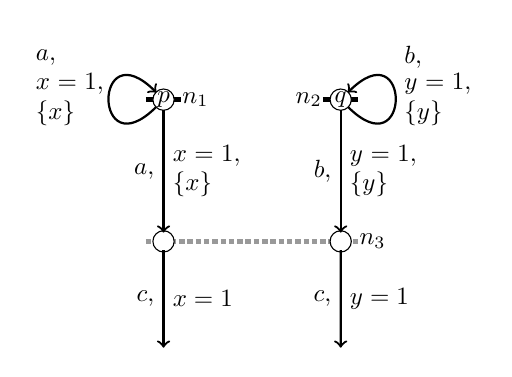
\begin{tikzpicture}[scale=0.9, every node/.style={transform shape}]

\begin{scope}[line width=2pt]
\draw (-.25,0) -- (0.25,0);
\draw (2.25,0) -- (2.75,0);
\draw [opacity=0.4, densely dotted] (-.25,-2) -- (2.75,-2);
\end{scope}

\filldraw [fill=white]  (0,0)  circle (1.5mm) node (pa) {$p$};
\filldraw [fill=white]  (2.5,0)  circle (1.5mm) node (qb) {$q$};
\filldraw [fill=white]  (0,-2)  circle (1.5mm) node (pc) {};
\filldraw [fill=white]  (2.5,-2)  circle (1.5mm) node (qc) {};

\node at (0.45,0) {$n_1$};
\node at (2.05,0) {$n_2$};
\node at (2.95,-2) {$n_3$};
\node at (-1.3,0.6) [text width=1cm] {$a,$};
\node at (3.9,0.6) [text width=1cm] {$b,$};
\node at (-1.3,0) [text width=1cm] {$x=1,$ $\{x\}$};
\node at (3.9,0) [text width=1cm] {$y=1,$ $\{y\}$};

\begin{scope}[thick,->]
\draw (pa) + (0,-.14) -- (pc) node [midway, left] {$a,$} node [midway, right, text width=1cm] {$x=1,$ $\{x\}$};
\draw (qb) + (0,-.14) -- (qc) node [midway, left] {$b,$} node [midway, right, text width = 1cm] {$y=1,$ $\{y\}$};
\draw (pc) -- (0,-3.5) node [midway, left] {$c,$} node [midway, right, text width=1cm] {$x=1$};
\draw (qc) -- (2.5,-3.5) node [midway, left] {$c,$} node [midway, right, text width=1cm] {$y=1$};
\draw (-0.1,-0.1) .. controls (-1,-1) and (-1,1) .. (-0.1,0.1);
\draw (2.6,-0.1) .. controls (3.5,-1) and (3.5,1) .. (2.6,0.1);
\end{scope}

\end{tikzpicture}
\caption{A local-timed negotiation depicting that the untimed
          language of the outcome sequences need not be regular. The
          synchronizing node $n_3$ forces the number of $a$s and number of $b$s to be equal.}

	\label{fig:abc}
\end{figure}

\section{Comparison with related models}

\section{Reachability is undecidable for local-timed negotiations}

When we allow both synchronized and unsynchronized nodes, we are
unable to use either of the techniques of the previous two
sections. In fact, reachability
turns out to be undecidable. Since local-times are independent of each
other, it is possible to have an unbounded drift between the reference
clocks of two agents. This helps store counter values as differences
between the local times. The main challenge is the check for
zero. This is where we require a combination of synchronized and
unsynchronized interactions. We will now show how to simulate a counter
machine using a local-timed negotiation.

\begin{theorem}\label{thm:undecidability}
  Location-reachability is undecidable for local-timed negotiations.
\end{theorem}

The rest of the section is devoted to proving
Theorem~\ref{thm:undecidability}. We will encode the halting problem
of a $2$-counter machine as the reachability problem for a local-timed
negotiation.


\noindent \emph{Counter machines.} A $2$-counter machine $M$ is a program that manipulates two counters, $C_1$ and $C_2$,
each of which can hold a non-negative number. The machine is given as
a sequence of labelled instructions $\ell:I$, where $I$ is one of the following for some $i \in \{1, 2\}$: 
\begin{description}
\item[increment] $C_i + +$, which increments the value of the
  counter $C_i$ and goes to the next instruction
  $\ell+1$.
\item[decrement] if $C_i>0$ then $C_i- -$, which decrements $C_i$ and continues with the next instruction
  $\ell+1$. If the value of $C_i$ is $0$, then the program is blocked. 
\item[jump-on-zero] if $C_i= = 0$ goto $\ell'$, which transfers control to the instruction labelled $\ell'$ if counter $C_i$ is $0$ for
  $i\in\{1,2\}$. If $C_i>0$, it continues to the instruction $\ell+1$.
\end{description}
The counter machine is said to halt if it reaches the final
instruction. A configuration of $M$ is a triple $(\ell, c_1, c_2)$ representing the current instruction $\ell$ that needs to be executed and the current values $c_1, c_2 \ge 0$ of the counters $C_1, C_2$ respectively. The transitions $(\ell, c_1, c_2) \xra{} (\ell', c'_1, c'_2)$ follow naturally from the description above.


\noindent \emph{Overview of the reduction.} The negotiation $\Nn_M$ that we
construct will have $6$ agents $p_1, q_1, r_1, p_2, q_2, r_2$. Agents
$p_1, q_1, r_1$ simulate counter $C_1$, and the rest simulate
$C_2$. Let $i \in \{1, 2\}$. The local clocks of $p_i, q_i, r_i$ are
respectively $\{x_{p_i}\}$, $\{x_{q_i}, x'_{q_i}\}$ and $\{x_{r_i}\}$. Additionally, we have the reference clocks $t_\a$ for each agent $\a$. For every instruction $\ell$, we will have a node
$n_\ell$ in which all the six agents participate.
A configuration $(C, v)$ of $\Nn_M$ is said to encode configuration
$(\ell, c_1, c_2)$ of $M$ if:
\begin{itemize}
\item $C(\a) = \{n_\ell\}$ for every agent $\a$,
\item $v(x) = 0$ for all local clocks (and reference clocks can take any value),
\item $v(t_{r_1}) \le v(t_{q_1}) \le v(t_{p_1})$ and $v(t_{r_2}) \le v(t_{q_2}) \le v(t_{p_2})$, and 
\item $v(t_{p_1} - t_{q_1}) = c_1$ and $v(t_{p_2} - t_{q_2}) = c_2$,
\end{itemize}
The initial configuration of $\Nn_M$ has every agent in $n_{\ell_0}$, where $\ell_0$ is the first instruction in $M$ and every clock (including reference clocks) to be $0$.

We will have a gadget in $\Nn_M$ corresponding to each instruction in the counter machine. Let $(C, v), (C',v')$ be configurations that encode $(\ell, c_1, c_2)$ and $(\ell', c'_1, c'_2)$ respectively. A run $(C, v) \xra{} \cdots \xra{} (C', v')$ such that none of the intermediate configurations encodes any counter machine configuration will be called a \emph{big step}. We denote a big step as $(C, v) \Rightarrow (C', v')$. Our gadgets will ensure the following two properties.
\begin{itemize}
\item Let $(\ell, c_1, c_2) \xra{} (\ell', c'_1, c'_2)$ in $M$. Then from every configuration $(C, v)$ that encodes $(\ell, c_1, c_2)$, there is a big step $(C, v) \Rightarrow (C', v')$ to some configuration $(C', v')$ that encodes $(\ell', c'_1, c'_2)$.
\item Let $(C, v), (C', v')$ be arbitrary configurations of $\Nn_M$ that encode $(\ell, c_1, c_2)$ and $(\ell', c'_1, c'_2)$ respectively. If $(C, v) \Rightarrow (C', v')$ is a big step, then $(\ell, c_1, c_2) \xra{} (\ell', c'_1, c'_2)$ in $M$.
\end{itemize}
The first property ensures that for every path $(\ell^0, c^0_1, c^0_2)
\xra{} (\ell^1, c^1_1, c^1_2) \xra{} \cdots$, there is a sequence of
big steps $(C_0, v_0) \Rightarrow (C_1, v_1) \Rightarrow \cdots$ such
that  $(C_i, v_i)$ encodes $(\ell^i, c^i_1, c^i_2)$. The second
property ensures the reverse: from a sequence of big steps, we get
a corresponding run in counter machine. We will now describe each
gadget and show that the two properties are satisfied.  

\begin{figure}[t]
\begin{center}
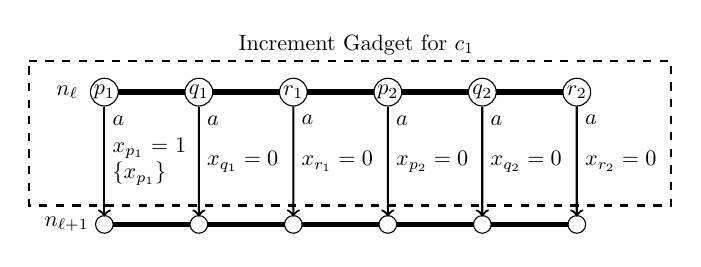
\begin{tikzpicture}[scale=0.8, every node/.style={transform shape}]

\begin{scope}[line width=2pt]
\draw (0,0) -- (7.5,0);
\draw (0,-2.1) -- (7.5,-2.1);
\end{scope}

\filldraw [fill=white]  (0,0)	  circle (2.2mm) node (nip1) [label={left:$n_{\ell}$}] {$p_1$};
\filldraw [fill=white]  (1.5,0)	  circle (2.2mm) node (niq1) {$q_1$};
\filldraw [fill=white]  (3,0)	  circle (2.2mm) node (nir1) {$r_1$};
\filldraw [fill=white]  (4.5,0)	  circle (2.2mm) node (nip2) {$p_2$};
\filldraw [fill=white]  (6,0)	  circle (2.2mm) node (niq2) {$q_2$};
\filldraw [fill=white]  (7.5,0)	  circle (2.2mm) node (nir2) {$r_2$};
\filldraw [fill=white]  (0,-2.1)	  circle (1.4mm) node (n2p1) [label={left:$n_{\ell + 1}$}] {};
\filldraw [fill=white]  (1.5,-2.1)	  circle (1.4mm) node (n2q1) {};
\filldraw [fill=white]  (3,-2.1)	  circle (1.4mm) node (n2r1) {};
\filldraw [fill=white]  (4.5,-2.1)	  circle (1.4mm) node (n2p2) {};
\filldraw [fill=white]  (6,-2.1)	  circle (1.4mm) node (n2q2) {};
\filldraw [fill=white]  (7.5,-2.1)	  circle (1.4mm) node (n2r2) {};

\begin{scope}[thick,->]
  \draw (nip1) -- node [very near start, right] {$a$} (n2p1)	 node [midway,right, text width=1.25cm] {$x_{p_1}=1$ $\{x_{p_1}\}$};
  \draw (niq1) -- node [very near start, right] {$a$} (n2q1)	 node [midway,right, text width=1.25cm] {$x_{q_1}=0$};
  \draw (nir1) -- node [very near start, right] {$a$} (n2r1)	 node [midway,right, text width=1.25cm] {$x_{r_1}=0$};
  \draw (nip2) -- node [very near start, right] {$a$} (n2p2)	 node [midway,right, text width=1.25cm] {$x_{p_2}=0$};
  \draw (niq2) -- node [very near start, right] {$a$} (n2q2)	 node [midway,right, text width=1.25cm] {$x_{q_2}=0$};
  \draw (nir2) -- node [very near start, right] {$a$} (n2r2)	 node [midway,right, text width=1.25cm] {$x_{r_2}=0$};
\end{scope}

\draw [dashed, thick] (-1.2,0.5) -- (9,0.5) -- (9,-1.8) -- (-1.2,-1.8) -- (-1.2,0.5);

\node at (4,.75) {Increment Gadget for $c_1$};
\end{tikzpicture}
\caption{Gadget for implementing increment instruction on $c_1$}
\label{fig:increment}
\end{center}
\end{figure}


\noindent \emph{Increment.} Assume an instruction $\ell: C_1 ++$ with $\ell$ not being the final instruction. The case with $C_2++$ is symmetric. Every configuration $(\ell, c_1, c_2)$ on executing this instruction goes to $(\ell + 1, c_1 + 1, c_2)$. Figure~\ref{fig:increment} shows the gadget for the increment instruction. All agents other than $p_1$ cannot elapse time due to the guard checking local clocks to $0$. Agent $p_1$ elapses
exactly one time unit, after which clock $x_{p_1}$ is reset.
It is easy to see that the configuration $(C', v')$ that results from $(C, v)$
encodes $(\ell', c_1 + 1, c_2)$. The big step $(C, v) \Rightarrow (C',v')$ is in fact a single transition. Both the properties are easily seen to be satisfied. 

\includegraphics{decrement-gadget.pdf}

\paragraph*{Decrement.} Consider a decrement instruction: if $C_1 > 0$
then $C_1 --$. We have
$(\ell, c_1, c_2) \xra{} (\ell+1, c_1 - 1, c_2)$ if $c_1 > 0$. The
first task is to check if $c_1 > 0$. Recall that in the negotiation the difference $t_{p_1} - t_{q_1}$ gives the value of $c_1$. Our idea is to let $q_1$ elapse time to
synchronize with $p_1$ and check if this time elapse needed for
synchronization is strictly above $0$ or not. However, in this
process, we lose the actual value of the counter. In order to maintain the same difference between $t_{p_1}$ and $t_{q_1}$, we make use of the auxiliary process $r_1$.

Consider a configuration $(C, v)$ that encodes $(\ell, c_1, c_2)$. By our definition, $v(t_{r_1}) \le v(t_{p_1})$ and $v(t_{p_1} - t_{q_1}) = c_1$. 
\begin{itemize}
 
\item We first let $r_1$ synchronize with $p_1$, while $p_1$
  elapses no time.
\item Next, we keep moving both $p_1$ and $q_1$ by $1$ unit each until
  $q_1$ synchronizes with $r_1$. In this entire process $r_1$ is not
  allowed to elapse time.
\end{itemize}
By the end of this, we will get a valuation $v'$ with the same difference $v'(t_{p_1} - t_{q_1}) = c_1$
since both the agents were moved by the same amount. Moreover, we can
use an additional clock to check whether in the process of $q_1$
synchronizing with $r_1$, a non-zero time had elapsed in $q_1$.

The gadget is depicted in Figure~\ref{fig:jump-decrement}. For simplicity, we do not index the intermediate nodes $n_1, n_2, n_3, n_4$ by $\ell$. The computation proceeds in three phases. Below, we show the run of $\Nn_M$ along this gadget, restricted to the agents $p_1, q_1, r_1$. The other three agents simply move to the next possible instruction (this is not shown in the figure for simplicity). 

\smallskip

\noindent \emph{Phase 1.} Synchronize $r_1$ with $p_1$ maintaining no time
elapse in $p_1$ as follows: $((n_\ell, n_\ell, n_\ell), v) \xra{}
((n_1, n_2, n_1), v_1) \xra{} ((n_2, n_2, n_3), v_3)$. After the last
action, agents $p_1$ and $r_1$ are synchronized, that is,
$v_3(t_{p_1}) = v_3(t_{r_1})$. This is due to the node $n_1$ being a
synchronization node. Moreover, $v_3(t_{p_1}) = v(t_{p_1})$, due to
the guard $x_{p_1} = 0$. Similarly, $v_3(t_{q_1}) = v(t_{q_1})$ due to
$x_{q_1} = 0$.

\smallskip

\noindent \emph{Phase 2.} Move $p_1$ and $q_1$ repeatedly by one unit each:  $((n_2, n_2, n_3), v_3) \xra{b} ((n_2, n_2, n_3), v_3^1) \xra{b} \cdots \xra{b} ((n_2, n_2, n_3), v_3^k)$. By the end of $k$ iterations of $b$, we have $v^k_3(t_{p_1}) = v(t_{p_1}) + k$ and $v^k_3(t_{q_1}) = v(t_{q_1}) + k$.

\smallskip

\noindent \emph{Phase 3.} Check if the reference clocks of $q_1$ and $r_1$
are equal: $((n_2, n_2, n_3), v_3^k)$
$\xra{a} ((n_4, n_3, n_3), v_4) \xra{c} ((n_4, n_4, n_4), v_5)$. The
outcome $c$ at $n_4$ can be fired only if the reference clocks of
$q_1$ and $r_1$ are equal: that is, $v_4(t_{q_1}) = v_4(t_{r_1})$. Due
to the guard checking for $0$ at $a$ and $c$, we have
$v_5(t_{q_1}) = v_4(t_{q_1}) = v_3^k(t_{q_1})$. From Phase 2, this
value equals $v(t_{q_1}) + k$. Secondly, notice that
$v_4(t_{r_1}) = v_3(t_{r_1})$, which from Phase 1 equals
$v(t_{p_1})$. From the equality $v_4(t_{q_1}) = v_4(t_{r_1})$, we get
$v(t_{q_1}) + k = v(t_{p_1})$.  This shows that
$k = v(t_{p_1}) - v({t_{q_1}})$. The number of times the loop $b$ is
done equals the difference between $t_{p_1}$ and $t_{q_1}$ at the
start of this gadget. If the number of $b$ iterations is more than
this value or less than this value, location $(n_3, c)$ cannot be
executed and the negotiation cannot proceed further. 


When action $c$ is done, the clock $x'_{q_1}$ holds the time between
$st$ and $c$ for agent $q_1$, and this is exactly $k$. If $k > 0$ the
value of $t_{q_1}$ is increased by $1$, resulting in the counter value
getting decremented and the agents move to the next instruction (shown
as the decrement gadget in the figure). Otherwise, the agents are sent
to a gadget from which there is no run (shown as the block gadget in
the figure).
Notice the interplay between synchronized and unsynchronized nodes in
this gadget. It is crucial that $n_2$ is unsynchronized, whereas
nodes $n_1, n_3$ need to be.

\includegraphics{jump-gadget.pdf}

\noindent \emph{Jump-on-zero.} This gadget is similar to the decrement
gadget, where the first part was to check if $C_1$ is $0$ or not. When $C_1 == 0$, the gadget jumps to the
relevant instruction, otherwise it moves to the next instruction in
sequence. The gadget is shown in~\cite{mukund2023localtime}. 

\section{Conclusion}
\label{sec:conclusion}

We have presented a model of local-timed negotiations. This is
motivated by the need for expressing timing constraints between
interactions in a negotiation. We have chosen a local-time model and
incorporated a synchronization constraint as part of the model. We
have shown that reachability is decidable when there is no mix of
synchronized and unsynchronized interactions. This mix creates
situations where one agent needs to fire a number of outcomes before
synchronizing with a second agent, and in this process forces a third
agent to elapse time. We have used this in the gadget explained for
the decrement instruction. As future work, we would like to study
non-trivial restrictions which contain a mix of synchronized and
unsynchronized interactions and are yet decidable.

We would like to remark that such a synchronization constraint can be
added in the local-time semantics for networks of timed
automata. Currently, the local-time semantics forces every shared
action to be synchronized. The main reason is that the definition
gives equivalence with the global-time semantics for reachability and
B\"uchi reachability. For networks of timed automata, global-time
semantics is considered the gold standard. The local-time semantics is
studied as a heuristic to solve reachability and B\"uchi reachability,
since this has better independence properties and is therefore
amenable to partial-order methods.  In our case with negotiations, we
consider local-time as the original semantics and make synchronization
as an option to be specified in the model. This allows more
independence between the agents and makes it more attractive for
partial-order methods. Having a decidable fragment with controlled use
of synchronization would be interesting in this regard. 
